\chapter{Architecture du projet}
\section{Relations}
    Notre jeu est basé sur les relations entre les différentes parties qui composent notre environnement de jeu.   
    \subsection{Voisinage}
        Le voisinage d'une pièce correspond aux places du monde qui sont directement en contact avec la place de la pièce. Le nombre de voisins d'une pièce dépend donc de la géométrie de notre plateau (cf. \textbf{\ref{part:geometry}}). On va déterminer ces derniers en testant l'intégralité des directions disponibles pour la pièce en n'omettant pas de vérifier si les cases sont occupées ou non. Cela nous donne donc un ensemble de cases disponibles pour cette dernière qui répond bien aux contraintes géométriques du plateau.
        
    \subsection{Déplacements}
        Nos déplacements sont réalisés en modifiant dans le monde l'état de la position ainsi que l'index associé à la pièce en question. Cela informe donc aux autres pièces que cette position est prise et permet de savoir à quel joueur elle appartient.
        \medbreak
        Pour déterminer la position exacte du déplacement, on utilise un fonctionnement de recherche de proche en proche, qui va déterminer les voisins directs, puis en fonction du nombre de mouvements de la pièce, réefectuer ce processus avec le voisin direct situé de la direction souhaitée. Le déplacement de cette dernière se fait ensuite aléatoirement parmi ces possibilités et comme dit précédemment, il est impossible pour cette dernière de choisir une case déjà occupée par une pièce alliée. \\
        Nous avons choisi d'implémenter cette méthode de recherche de proche en proche car elle simplifie l'utilisation de variable de déplacement maximum pour chaque type de pièces.
        \medbreak
        \noindent Dans le cas où toutes les cases sont occupées par une pièce alliée, le joueur ne peut pas jouer et son tour est passé.
        
    \subsection{Changements de terrain}
        Dès lors que la partie commence, une initialisation de la \textit{seed} du terrain est nécessaire.
        \medbreak
        Cette \textit{seed} influe directement sur les interactions entre les différentes positions du monde et change donc les déplacements possibles. \\ Chaque pièce sera donc restreinte à un certain nombre de relations :
        \begin{itemize}
            \item Pour un terrain classique (hexagonal), toutes les directions sont autorisées.
            \item Pour un terrain à pavage triangulaire, une case sur deux possède les mêmes relations de voisinage, on a ici les relations (N,SE,SW) pour une partie des pièces et (S,NE,NW) pour l'autre.
            \item Pour un terrain à pavage carré, les seules directions autorisées sont celles des points cardinaux (N,S,E,W).
        \end{itemize}
        \medbreak
        Après avoir réduit le nombre de directions possible, le système de déplacement est appliqué de manière identique, elle prend alors compte des contraintes de direction.
        \medbreak
        \begin{figure}[H]
            \centering
            \begin{subfigure}{0.22\textwidth}
                \centering
                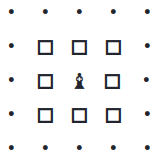
\includegraphics[scale= 0.35]{img/dep_hexagonal.png}
                \caption{Classique hexagonal}
                \label{fig:dep_hexa}
            \end{subfigure}
            \quad
            \begin{subfigure}{0.2\textwidth}
                \centering
                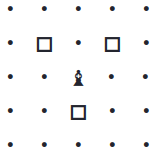
\includegraphics[scale= 0.35]{img/dep_triangle_1.png}
                \caption{Triangulaire 1}
                \label{fig:dep_tri1}
            \end{subfigure}
            \quad 
            \begin{subfigure}{0.2\textwidth}
                \centering
                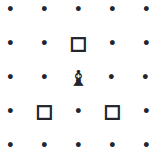
\includegraphics[scale= 0.35]{img/dep_triangle_2.png}
                \caption{ Triangulaire 2}
                \label{fig:de_triangulaire 2}
            \end{subfigure}
            \label{label_de_la_figure 3}
            \quad 
             \begin{subfigure}{0.2\textwidth}
                \centering
                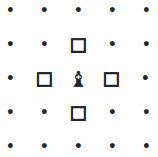
\includegraphics[scale= 0.35]{img/dep_carre.png}
                \caption{Carré}
                \label{fig:dep_carre}
            \end{subfigure}
            \caption{Les différents déplacements en fonction des pavages.}
        \end{figure}
        
        Nous avons donc réussi à implémenter un système qui en modifiant une \textit{seed} de terrain, modifie les relations de voisinage de la partie en cours.
    \subsection{Positions de départ}
        Etant donnés l'aspect torique de notre plateau, nous avons dû faire très attention aux déséquilibres possibles en début de la partie, et ceci beaucoup plus que pour un plateau classique où il aurait suffi de positionner les pièces de chaque côtés de celui-ci.

        C'est pour résoudre ce problème que nous avons décidé d'utiliser un algorithme pour créer les formations en fonction des paramètres. Pour cela, nous avons implémenté un algorithme qui en fonction des types de pièces à placer et de leur nombre, choisit une formation qui soit identique pour chaque joueur et qui ne crée pas de déséquilibre entre eux, et ceci quel que soit le nombre de joueurs ou la taille du plateau de jeu. Par exemple, la figure \textbf{\ref{fig:depart_classique_a_4}} montre les positions de départ pour une partie lancée avec 4 joueurs, sur un monde de taille $10\times10$, avec  $2$ tours (pièce, cf. \textbf{\ref{part:tower}}) par joueur.
            
        \begin{figure}[H]
            \centering
            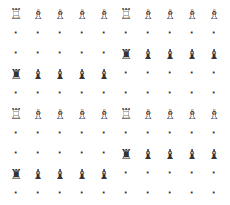
\includegraphics[scale=0.6]{img/depart_classique_a_4.png}
            \caption{Départ classique à 4}
            \label{fig:depart_classique_a_4}
        \end{figure}

        Cette facon de penser le départ du jeu nous a permis le rendre jeu encore plus modulable et de l'adapter à beaucoup plus de configurations en permettant des possibilités de départ presque infinies.
            
    \subsection{Capture et libération}
        Si une pièce atterit sur une pièce adverse, une capture est réalisée. Si plus tard, la position de la pièce capturée est libre, elle a une probabilité d'être libérée. Cette probabilité est fixée à \texttt{50/100} mais peut être modifiée par l'utilisateur. La question de la capture d'une pièce adverse par un joueur est une des raisons qui nous ont poussé à créer un "monde extérieur" (développé en \textbf{\ref{part:world_ext}}), qui sous forme d'une structre contient le plateau, les joueurs et les pions.
        \medbreak
        \noindent L'implémentation de cette structure nous a permis d'implémenter la capture de cette façon :
        \begin{itemize}
            \item[$\bullet$] Opérations sur la pièce :
            \begin{itemize}
                \item Lorsqu'une pièce est capturée, sont attribut \texttt{captured} (cf. \textbf{\ref{part:pawns}}) prend la valeur \texttt{1}.
            \end{itemize}
            \item[$\bullet$] Opération sur le monde extérieur :
            \begin{itemize}
                \item La pièce est ajoutée à la liste des pièces capturées : \texttt{captured\_pawns[]}, et sa position est retirée de la liste des positions prises par le joueur : \texttt{current\_sets[index\_du\_joueur][]}.
            \end{itemize}
        \end{itemize}
        \medbreak
        Procéder de cette manière nous a permis de ne pas modifier la position de la pièce capturée, ainsi, elle la garde en mémoire. Lorsque les conditions de libération sont remplies, on effectue le schéma inverse, et la pièce est de retour sur le plateau.
        \newpage

\section{Organisation et structure du projet}\

    \subsection{Organisation du monde}\label{part:world_ext}
        Afin de faire évoluer notre jeu tout en gardant un aspect modulaire, nous avons dû créer un fichier "monde extérieur", \texttt{world\_ext.c}, qui englobe la totalité des objets de notre jeu (monde, joueurs, pièces, ...).  Ce fichier implémente la structure suivante.

        \begin{lstlisting}
struct world_ext_t {
	struct world_t* world;                       // Plateau de jeu
	int nb_players;                              // Nombre de joueurs.
	struct players_t players[WORLD_SIZE];        // Liste des joueurs.
	struct sets_t initial_sets[WORLD_SIZE];      // Ensembles de positions de départ des
                                                 // joueurs.
	struct sets_t current_sets[WORLD_SIZE];      // Ensembles de positions prises par
                                                 // chaque joueurs.
	int nb_captured_pawns;                       // Nombre de pièces capturées.
	struct pawns_t* captured_pawns[WORLD_SIZE];  // Liste des pièces capturées.
};\end{lstlisting}

    Le fichier \texttt{world\_ext.c} met en lien l'ensemble des fichiers de base du jeu et fournit des fonctions \textit{de haut niveau} à la boucle de jeu, comme par exemple une fonction pour gérer les captures et les libérations, ou encore pour effectuer un déplacement de pièces.
    
    \subsection{Dépendances des fichiers}\label{part:graph_src}
        Afin de rendre le projet le plus modulable possible, nous avons séparé notre projet en plusieurs fichiers \texttt{.c}, ces fichiers contiennent les fonctions qui permettent au tout de fonctionner. Chacun de ces fichiers \texttt{.c} inclu un fichier \texttt{.h} du même nom. Ces fichiers d'entête contiennent les \texttt{header} de toutes les fonctions "publiques" qui ont pour but d'être utilisées par d'autres fichiers. Les inclusions ne se font jamais entre les fichiers \texttt{.c}, mais uniquement avec les \texttt{.h}.
        
        \begin{figure}[H]
            \centering
            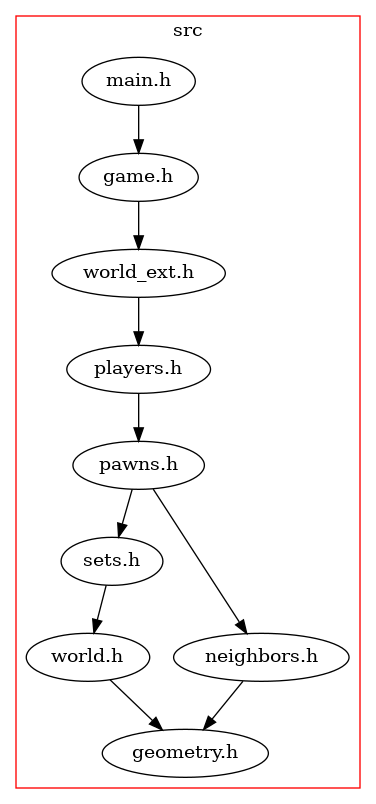
\includegraphics[scale=0.4]{img/graph_src.png}
            \caption{Graphique de dépendance des fichiers source. \textit{Généré avec} \texttt{Graphviz}.}
            \label{fig:graph_src}
        \end{figure}

        Cette organisation du projet à base d'inclusions nous permet une très grande modularité. En effet, si un fichier \texttt{.c} est modifié (comme par exemple \texttt{world.c}), le projet continue de fonctionner tant que la nouvelle implémentation respecte le fichier \texttt{.h} correspondant.

    \subsection{Compilation}
        Pour faciliter les travaux de compilations séparés, nous avons intégré un fichier \texttt{Makefile}. Ce fichier nous a permis de déclarer des règles générales qui simplifient les commandes de compilations. Nous nous en somme par exemple servi pour compiler automatiquement tous les fichiers \texttt{.o} nécessaires, ou encore pour compiler et éxécuter tous les tests en même temps.

\section{Tests}
    \subsection{Structure des tests}
        Nous avons décidé de séparer les tests dans différents fichiers pour plus de flexibilité. Chaque fichier test contient les fonctions visants à tester un unique fichier source. Cette méthode nous a permis de pouvoir tester l'ensemble du code source en même temps, ou bien de lancer les tests d'un fichier en particulier.

        \begin{figure}[H]
            \centering
            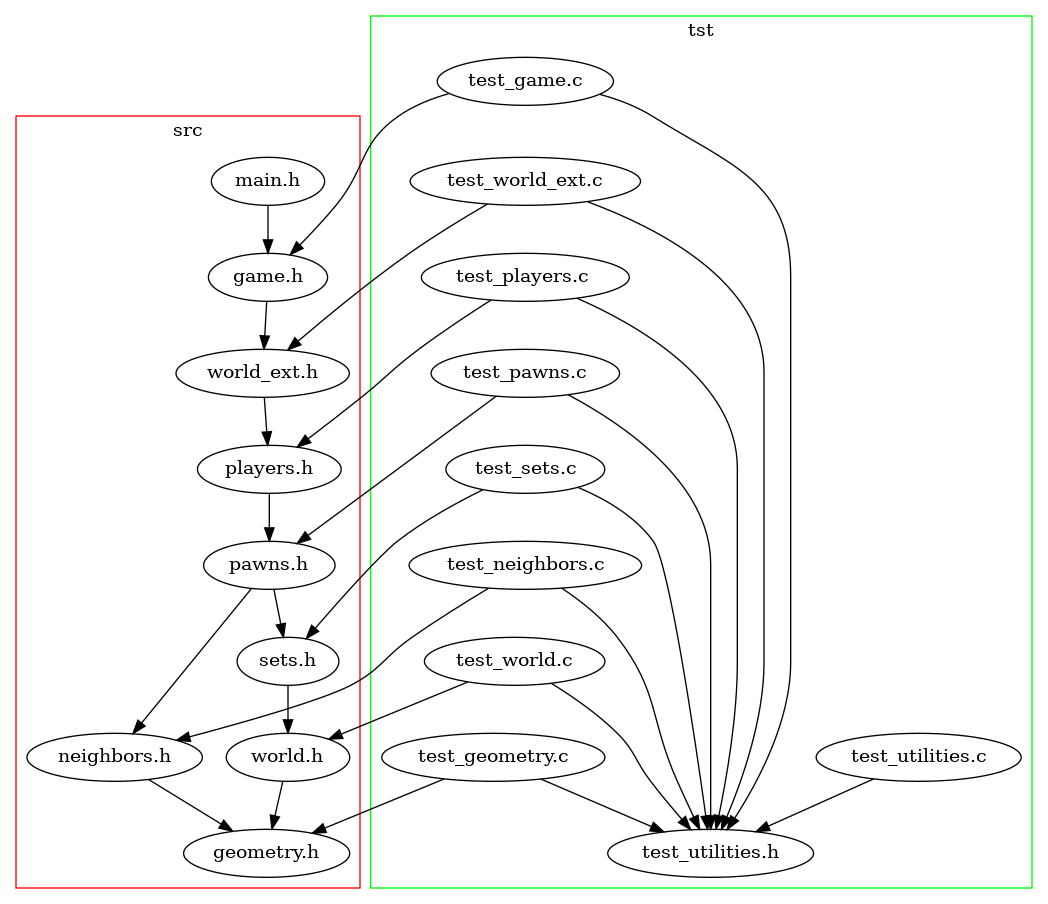
\includegraphics[scale=0.4]{img/graph_tst.png}
            \caption{Graphique de dépendance des fichiers tests. \textit{Généré avec} \texttt{Graphviz}.}
            \label{fig:graph_tst}
        \end{figure}

        \newpage

        La figure \textbf{\ref{fig:graph_tst}} montre les inclusions de nos fichiers tests. On remarque que chaque fichier test inclu uniquement le fichier source qu'il teste. De plus, nous avons décidés de séparer deux fonctions générales des tests dans un fichier \texttt{test\_utilities.c}. Ce fichier est le seul des fichiers tests à avoir un fichier d'entête, car c'est le seul qui est inclu dans d'autres fichiers. Il contient les deux fonctions suivantes :
        
        \begin{lstlisting}
void str_test(const char str1[], const char str2[]) // Compare 2 strings
{ 
    (!strcmp(str1, str2)) ? printf("\t\tPASSED\n") : printf("\t\tRecieve %s instead of %s.\n", str1, str2);
}

void int_test(const int int1, const int int2) // Compare 2 integers
{
    (int1 == int2) ? printf("\t\tPASSED\n") : printf("\t\tRecieve %d instead of %d.\n", int1, int2);
}\end{lstlisting}

        Ces deux fonctions nous ont été très utiles dans le cadre de la \textbf{programmation par le test}. En effet, appeler celles-ci dans nos fichiers test nous a permis de très facilement comparer les retours des fonctions testées avec ce que nous attendions. En cas de réussite, le programme affiche : \texttt{PASSED}, tandis que si le test ne passe pas, le programme affiche : \texttt{Recieve <valeur\_reçu> instead of <valeur\_attendue>}.
        \medbreak
        Nous avons donc pu écrire nos tests, puis implémenter nos fonctions jusqu'à ce que toute nos lignes de tests affichent : \texttt{PASSED}.
        

        
    